\documentclass{article}
\usepackage[utf8]{inputenc}
\usepackage[margin=2.6cm]{geometry}
\usepackage{float}
\usepackage{rotating}
\usepackage{graphicx}
\usepackage{caption}
\usepackage{subcaption}
\usepackage[round]{natbib}
\usepackage{setspace}
\usepackage{longtable}
\usepackage{lscape}
\onehalfspacing
\usepackage{tikz}
\usetikzlibrary{arrows,automata,positioning,shapes}

\title{The interplay of resource acquisition and transfers explains the diversity of the female human life cycle.
\\
Registered Report}
\author{Pablo J. Varas Enriquez, Monique Borgerhoff Mulder, Heidi Colleran, Dieter Lukas*\\\\
* No special order of authors}
\date{\today}

\begin{document}

\maketitle

\tableofcontents

\section{Problem Formulation}

There are many developmental paths an individual can follow through its life cycle, which is the basis of the diversity seen across the tree of life. The diversity of reproductive schedules can go from a couple to thousands offspring (e.g. eastern hemlock vs rain moth \citep{tindale1932revision,van2017lifetime} and mortality ones from lifespans of days to thousands of years (e.g. hairyback vs patagonian cypress \citep{balsamo1988life,lara19933620}). The differences in life cycles have usually been related to the ways in which an individual allocates the limited resources it posses in its environment \citep{stearns2000life}. Female humans pose an interesting case regarding its life cycle due to the short reproductive period in comparison to their long lifespan, framed within long juvenile and post-reproductive stages \citep{kaplan2000theory}. Within these boundaries, female humans present a high diversity of life cycles across populations, where life spans can be long and their reproductive output low (e.g. post-demographic transition Japan \citep{de2017maximum}) while other populations have short lifespans and high reproductive output (e.g. foraging populations \citep{migliano2007life}). The high diversity of female life cycles among human populations is fuelled by the differences in longevity and fertility schedule between individuals within a population. While the differences in longevity at an individual level has been associated with resource acquisition (i.e. more resources equals longer lifespans) \citep{kaplan2003embodied}, the relationship of resource acquisition with fertility is more complex \citep{mulder1998demographic,sear2016understanding}. Additionally, resource transfers have been proposed as a way to understand the different life cycles among female humans. Here, the presence or different members of the population in the social network of a female individual have been associated with different life cycles \citep{sear2011much}. Examples can be found in literature related to cooperative breeding, sibling competition, female conflict, among others \citep{ivey2000cooperative,nitsch2013elder,mace2012female}. However, both frameworks usually focus on a) specific components of the life cycle (e.g. longevity, number of offsprings) and/or b) black box the ways in which resources are available for a female individual. The main evolutionary models that have tried to tackle these two aspects can be summarized in the embodied capital models and the resource transfer models. The embodied capital theory suggests that the surplus of resource production during adulthood allows the evolution of the female human life cycle \citep{kaplan2000theory}. This model proposes that the difference between resource production and consumption allows high parental investment, translated in short interbirth intervals and long post-reproductive periods for the parents and long juvenile periods for their offspring. Furthermore, the pooled energy model deepens in this framework by suggesting that alloparenting from individuals of different generations would allow to decrease the load of parental investment \citep{kramer2010pooled}. Resource transfer theory poses that inter-generational transfers would play a major role in the mortality and fertility schedules of human populations. \cite{lee2003rethinking} suggests that age-specific mortality is proportional to the remaining reproductive value and resource transfers made at later ages, predicting the early-life and later-life mortality patterns characteristics of the female human life cycle. Additionally, \cite{chu2006co} model shows that inter-generational transfers co-evolve with low mortality, since adults are more efficient to produce energy, which is transferred to juveniles, who are more efficient to turn that energy into body size, allowing lower mortality. Hence, these models show that the female human life cycle evolves from the interplay of resources acquisition and transfers. However, they do not explain the conditions under which the life cycle varies within a population nor completely address the influence of the different resource dynamics, as our model aims to do (see Fig.\ref{fig:1} for a graphical summary).

Therefore, this project aims to develop a theoretical framework to understand a) individual-level variations in the different components that characterize the female human life cycle (i.e. survival, age at menarche, age at first reproduction, number of offspring, interbirth intervals, age at last reproduction, age at menopause, longevity), and b) how these variations might be caused by different resource dynamics (i.e. resource production, consumption, transfer, storage) across the life cycle. The framework will be developed with agent-based models and will be described using an ODD (Overview, Design concepts, Details) protocol, as an standardised way to clarify the scope, assumptions, and parameters used to answer our questions \citep{grimm2006standard,grimm2020odd}.

\section{Model description}

\subsection{Purpose}

The female human life cycle is characterised by a long lifespan, within which there is usually a short reproductive period in between long juvenile and post-reproductive stages. Longevity, the boundaries of the reproductive period, and the frequency at which births occur during this period, are influenced by allocation of resources made by the individual. Previous work has linked variations in the life cycle of a female individual to the amount of resources available in the environment or the availability of a network of potential helpers, but how the interplay of both of them change the allocation of resources of an individual, and variations in its life cycle as consequence, remains unclear. Here we will develop a theoretical framework to understand how the interplay of resource acquisition and their sharing across the social network influence the variations of female life cycles within a population. More specifically, the model would allow identify which resource dynamics vary the timing of life stage transitions, longevity, and reproductive timing and output of individuals.
\\\\
For the purpose of this model, the life cycle of a female individual will be described by the time spent across five discrete stages (i.e. infant, juvenile, adult, reproductive-career, post-reproducitve), which are defined by the timing of key events of the life course (i.e. age at menarche, age at first reproduction, age at menopause, and death). Longevity will also be a characteristic of the life cycle (i.e. number of years alive), as well as lifetime reproductive success (i.e. number of surviving offspring until sexual maturity). The influence of resource dynamics into the life cycle will be understood by the timing of reproductive events (i.e. age at first and last reproduction, and interbirth intervals) and life stage transitions (i.e. age at menarche, age at first reproduction, age at menopause). Finally, resource dynamics will be characterized by the amount of resources produced, transferred, consumed, and stored in each life cycle stage. A graphical representation can be seen in Fig. \ref{fig:2}.

\subsection{Entities, state variables, and scale}

\subsubsection{Entities}

Individuals represent females in a single-sex, haploid population. Individuals that are born until they reach \emph{age at transition trait} are considered infants. Juveniles are individuals that transition from infants, until they reach age at menarche. Adults are individuals that have reached menarche until they have their first offspring or reach menopause. Adults transition to a reproductive-career stage once they have their first offspring, and remain in this stage until they reach menopause. From menopause onward individuals are considered post-reproductive.

\subsubsection{State variables}

Every individual in the simulation is characterised by state variables that are a) calculated new in each iteration, and b) modified from one iteration to the next:

\begin{itemize}
    \item Variables that are calculated new in each iteration:
    \begin{itemize}
        \item Resources produced: Amount of resources produced by the individual. The amount is fixed to each stage. Therefore, the individual whether produce resources (stage-specific resource production) or not (0) based on a stage-specific production probability specified during initialisation.
        \item Resources received: Amount of resources received by the individual from other individual(s). The amount received by another individual is fixed to each stage. Therefore, the individual receives resources depending on the number of times the stage-specific probability is successful ($1$) or not ($0$), constrained by the stage-specific number of times receiving specified during initialisation.
        \item Resources consumed: Amount of resources consumed by the individual. The amount is fixed to each stage and specified during initialisation.
        \item Resources gave: Amount of resources given by the individual to other individual(s). The amount given to another individual is fixed to each stage. Therefore, the individual gives resources depending on the number of times the stage-specific probability is successful ($1$) or not ($0$), constrained by the stage-specific number of times giving specified during initialisation.
        \item Reproductive effort: Amount of resources the individual uses for reproduction, given the stage-specific probability. The amount is fixed to each stage. Therefore, the individual whether gives birth ($1$)  or not ($0$) based on the stage-specific fertility probability and the amount of resources produced, received, consumed, gave, and stored.
    \end{itemize}
    \item Variables that are modified from one iteration to the next:
    \begin{itemize}
        \item Age: Amount of iterations the individual goes through from its birth until it dies. Age increases by one after each iteration, reflecting one year.
        \item Stage: Life cycle stage in which the individual is at the moment. There are five stages (infant, juvenile, adult, reproductive-career, post-reproductive), each with its own stage-specific resource and life-history dynamics. Individual progression through the stages is determined by the allocation of resources in the key event of transition.
        \item Resources stored: Amount of resources the individual stores for later in time (i.e. next iteration). The amount of resources stored depends on the surplus resources after the stage-specific resource and life-history dynamics. Therefore, the individual whether stores the surplus (stage-specific storing) or loses it (0) based on the stage-specific storing probability.
        \item Reproductive output: Amount of offsprings produced, given the stage-specific fertility probability. Reproductive output increases by one after an iteration, if reproductive requirements (i.e. fertility probability and resources available) are met.
    \end{itemize}
\end{itemize}

\subsubsection{Auxiliary variables}

The individual dynamics are constrained by the following auxiliary variables. These variables are stage-specific, set at the initialisation and apply to all individuals in dependence on their state variables.

\begin{itemize}
    \item Die: Probability of dying in the life cycle stage. The probability distribution is based on the mortality rates from the cross-cultural study by \cite{gurven2007longevity}, which is adjusted according to the resources available for an individual.
    \item Produce: Probability of producing resources. The probability is based on a binomial distribution regarding whether the individual produces resources ($1$) or not ($0$). The values of the distribution are based on \cite{koster2020life}.
    \item Times receiving: Number of individuals from whom receiving resources. The values can go from zero to the maximum number of individuals available for giving in the cross-cultural study by \cite{gurven2004give}, constrained by population size.
    \item Receive: Probability of receiving resources from another individual. The probability is based on a binomial distribution regarding whether the individual receives resources ($1$) or not ($0$). The values of the distribution are based on \cite{gurven2004give}. The sampling size is defined by \emph{Times receiving}.
    \item Consume: Amount of resources necessary for somatic maintenance, based on \cite{kaplan2000theory,pontzer2021daily}.
    \item Store: Probability of storing the surplus of resources from production and sharing dynamics at the end of an iteration. The probability is based on a binomial distribution regarding whether the individual stores resources ($1$) or not ($0$). The values of the distribution are based on \citep{bowles2011cultivation}.
    \item Times giving: Number of times giving resources from other individual(s). The values can go from zero to the maximum number of individuals available for receiving in the cross-cultural study by \cite{gurven2004give}, constrained by population size.
    \item Give: Probability of giving resources to another individual. The probability is based on a binomial distribution regarding whether the individual gives resources ($1$) or not ($0$) . The values of the distribution are based on \cite{gurven2004give}. The sampling size is defined by \emph{Times giving}.
    \item Reproduce: Probability of producing a offspring. The probability is based on a stage-specific fertility rate, which is adjusted according to the resources available for an individual.
    \item Transition: Probability of transitioning to the next stage. The transitions are specified as follow:
    \begin{itemize}
        \item Infant transition: Reaching the growth and development necessary to transition to the juvenile stage.
        \item Sexual maturity: Reaching the development necessary for menarche and transition to the adult stage. The probability distribution is based on the values in \cite{mulder1989menarche} and \cite{kramer2010teen}.
        \item Reproduce (adult stage): Producing your first offspring and transition to the reproductive-career stage. The values of the distribution are based on the work of \cite{wood2017dynamics}.
        \item Menopause: Reaching the moment where you cannot, biologically, produce more offspring and transition to the post-reproductive stage. The values of age at menopause are based on \cite{laisk2019demographic}.
    \end{itemize}
\end{itemize}

\subsubsection{Scale}

Each iteration in the model represents one year. The probabilities  of producing, receiving, consuming, giving, and storing are binomial, with the values of happening ($1$) or not ($0$). The amount of resources an individual produces, receives, consumes, gives, and store are stage-specific. The number of times an individual receives and gives are also stage-specific. Reproductive effort is evaluated after the resource dynamics, followed by the evaluation for stage transition. Finally, the amount or resources available are stored and passed from one year to the next, being evaluated for survival at the beginning of the iteration.

\subsection{Process overview and scheduling}

Every sub model described in the following process is stage-specific. Infant individuals go through survival, receiving, consuming, and storing sub models each year until they transition to the next stage. Once in the juvenile stage, individuals go through survive, produce, receive, consume, give, and store sub models for each year until they reach sexual maturity, transitioning to the adult stage. In the adult stage, individuals go through surviving, producing, receiving, consuming, giving, and storing sub models until they have their first offspring or reach menopause. If an adult transition to a reproductive-career stage, it goes through surviving, producing, receiving, consuming, giving, storing sub models and also through a reproduction sub model until it reaches menopause. Once in a post-reproductive stage, the individual goes through the surviving, producing, receiving, consuming, giving, and storing sub models of the stage. In each year, the individual increase its age and updates they amount of resources it has. During each transition, the individual updates its stage variable and also transitions with the resources it has stored from the earlier stage.
\\\\
The scheduling of the process starts with the survival sub model so only individuals who survive can age and go through the rest of the sub models in the iteration. The resource-related sub models start with those who may increase the amount of resources available (production and receiving), followed by those who decrease the amount of resources (consumption and giving), and ending with the storing sub model. The reproduction sub model follows the resource-related ones in order to see the influence of resource dynamics in the reproductive output and timing. The schedule ends with the transition sub model to evaluate if the individual moves to the next life cycle stage or not.

\subsection{Design concepts}

\subsubsection{Basic principles}

The model aims to offer a theoretical framework to understand the variability of life cycles within a human population, by understanding the role of resource acquisition and transfers, combined, in the timing and output of reproduction and survival. Evolutionary models have focused on the evolution of the human life cycle, and its characterisation of having a long lifespan where a short reproductive-career develops between long juvenile and post-reproductive stages. However, understanding how the female human life cycle varies might shed some lights on the different pathways under which the human life cycle has evolved. Here, the embodied capital theory \citep{kaplan2000theory} and the pooled energy model \citep{kramer2010pooled} focus on the surplus of energy available to allocation in survival and fertility due to differences between resource production and consumption, as well as transfers from alloparenting. Resource transfer models \citep{lee2003rethinking,chu2006co} explore the sharing dynamics and their relationship with the evolution of the human life cycle, where downwards inter-generational transfers predict early-life and later-life mortality patterns, especially low-mortality ones. Hence, these models show that the female human life cycle evolves from the interplay of resources acquisition and transfers. However, they do not explain the conditions under which the life cycle varies within a population nor completely address the influence of the different resource dynamics, as our model aims to do.

\subsubsection{Emergence}

The life cycle of an individual emerges from its behaviour. The life cycle is represented by the timing of key events of the life course (i.e. life stage transition, reproductive output and timing, and longevity) constrained by the stage-specific sub models related to resource dynamics. Population dynamics emerge from the behaviour of the individuals. The population dynamics are represented as the age distributions of the life cycle transitions, reproductive output and timing, and longevity and surviving individuals. The aim is to understand how the resource dynamics (i.e. production, consumption, transfer, storage) experienced by individuals within a population cause changes in the variability of different components of the female human life cycle (i.e. survival, age at menarche, age at first reproduction, number of offspring, interbirth intervals, age at last reproduction, age at menopause, longevity).

\subsubsection{Adaptation}

The model has three adaptive behaviours, that characterise the female human life cycle: 1) the time to transition from one life stage to another, 2) the reproductive output and timing, and 3) longevity. The three of them are based on whether the individual have a successful outcome from the different state variables as well as enough resources to allocate in survival and/or reproduction. An individual transitions, reproduces, and/or survives using an stochastic process described below in the corresponding sub models.

\subsubsection{Objectives}

The objective measures used by the individuals in the model to whether transition, reproduce, and/or survive are the amount of resources that the individual acquires from the different resource dynamics, as well as having a successful outcome from the different state variables. The mechanism to have a successful outcome is based on a stochastic process described below in the corresponding sub models.

\subsubsection{Learning}

There is no learning process for the individuals in the population because the model focuses on the biological constraints under which the female human life cycle varies.

\subsubsection{Prediction}

The variability of female life cycles within a human population would fluctuate depending on the different resource dynamics that individuals experience through their lives. On the one hand, variability should be higher in scenarios where individuals would have lower access to resources via receiving or production, less storage capacity, and/or give more resources to other individuals. On the other hand, there should be less variability of life cycles in a population where individuals would have higher access to resources via receiving or production, higher storage capacity, and/or give less resources to other individuals. Between these two extremes, the variability of female life cycles should be more sensitive to changes in resource production and consumption, whereas sharing and storing dynamics should have a buffering effect.

\subsubsection{Sensing}

Individuals are assumed to know their stage, and their current resources produced, consumed, received, gave, and stored in order to allocate them into reproduction, survival, and/or transitioning from one life cycle stage to another.

\subsubsection{Interaction}

Not apply

\subsubsection{Stochasticity}

Resource dynamics and the allocation of them towards different key components of the female human life cycle are stochastic in the model since they are based on probability distributions. Individuals produce, receive, consume, give, and store resources within an iteration based on having a successful outcome ($1$) from a binomial distribution, which is totally random. Individuals survive, reproduce, and transition from one life stage to another not automatically by reaching a certain amount of resources, they also need to have a successful outcome ($1$) from a binomial distribution to allocate those resources, which also is totally random. Therefore, decisions are stochastic within the constrains of resources available for the individual.

\subsubsection{Collectives}

Not apply

\subsubsection{Observation}

The purpose of the model is to identify which scenarios of resource acquisition and transfers vary the timing of life stage transitions, longevity, and reproductive timing and output of individuals. Therefore, the different resource dynamics (i.e. production, consumption, giving, receiving, storing) and the timing and output of the different components of the life cycle are recorded for each individual. At the population level, distributions of each trait of the female human life cycle as well as resource dynamics are produced based on the individual data.

\subsection{Initialization}

At initialisation, the population will be composed of equal number of individuals per life cycle stage. Each infant individual in the initial population have the baseline resources to survive to guarantee the survival in the first survival sub model and go through the resource dynamics sub models, only ageing after surviving the survival sub model in the next iteration.
\\\\
The auxiliary variables for each stage are set at initialisation. The values for each variable and stage are based on previous research (Table \ref{tab:1}).

\subsection{Input Data}

The model does not use input data to represent time-varying processes.

\subsection{Sub models}

Each individual goes through all the stage-specific sub models each iteration.

\begin{itemize}
    \item Infant
    \begin{itemize}
        \item Die: The infant survives by sampling a value equal or higher than the stage-specific survival rate, based on \cite{gurven2007longevity}. If the individual samples a value lower than the stage-specific survival rate, then it dies. The infant has a higher chance to survive if it has a larger amount of resources available. The amount of resources decreases by the costs of survival.
        \item Times receiving: The individual receives resources from a certain number of individuals. This is based on sampling a value between zero and the maximum number of givers in \cite{gurven2004give}, constrained by population size.
        \item Receive: The infant has a probability of receiving from another individual by sampling from a binomial distribution. The individual either receives resources ($1$) or not ($0$), and the amount of resources received per giver is fixed, stage-specific, and based on the \cite{gurven2004give}. The sample size is defined by the value from the \emph{Times receiving} sub model. 
        \item Consume: The infant consumes the amount of resources necessary for somatic maintenance from the resources the individual acquires from the sub models  \emph{Receive} and \emph{Store} in the iteration, based on \cite{kaplan2000theory, pontzer2021daily}.
        \item Store: The infant has a probability of storing the surplus of resources available in the iteration by sampling from a binomial distribution. The individual either stores ($1$) or not ($0$), based on the values on \citep{bowles2011cultivation}. In case the individual does not store ($0$) then the surplus  of resources in the iteration is lost.
        \item Transition: The infant transition by sampling a value equal or higher than the stage-specific probability of transition, based on the values on \emph{(ref. missing)}. The infant has a higher chance to transition if it has a larger amount of resources from the \emph{Receive} and \emph{Store} sub models. The amount of resources decreases by the costs of transition, while the remaining amount is stored, and transition to the juvenile stage.
    \end{itemize}
    \item Juvenile
    \begin{itemize}
        \item Die: The juvenile survives by sampling a value equal or higher than the stage-specific survival rate, based on \cite{gurven2007longevity}. If the individual samples a value lower than the stage-specific survival rate, then it dies. The juvenile has a higher chance to survive if it has a larger amount of resources stored from the previous iteration. The amount of resources decreases by the costs of survival.
        \item Produce: The juvenile has a probability of producing by sampling from a binomial distribution. The individual either produces resources ($1$) or not ($0$), and the amount of resources produced is fixed, stage-specific, and based on \cite{koster2020life}.
        \item Times receiving: The individual receives resources from a certain number of individuals. This is based on sampling a value between zero and the maximum number of givers in \cite{gurven2004give}, constrained by population size.
        \item Receive: The juvenile has a probability of receiving from another individual by sampling from a binomial distribution. The individual either receives resources ($1$) or not ($0$), and the amount of resources received per giver is fixed, stage-specific, and based on the \cite{gurven2004give}. The sample size is defined by the value from the \emph{Times receiving} sub model. 
        \item Consume: The juvenile consumes the amount of resources necessary for somatic maintenance from the resources available in the iteration, based on \cite{kaplan2000theory,pontzer2021daily}.
        \item Times giving: The individual gives resources from a certain number of individuals. This is based on sampling a value between zero and the maximum number of receivers in \cite{gurven2004give}, constrained by population size.
        \item Give: The juvenile has a probability of giving from another individual by sampling from a binomial distribution. The individual either gives resources ($1$) or not ($0$), and the amount of resources gave per receiver is fixed, stage-specific, and based on the \cite{gurven2004give}. The sample size is defined by the value from the \emph{Times giving} sub model. 
        \item Store: The juvenile has a probability of storing the surplus of resources available in the iteration by sampling from a binomial distribution. The individual either stores ($1$) or not ($0$), based on the values on \citep{bowles2011cultivation}. In case the individual does not store ($0$) then the surplus of resources in the iteration is lost.
        \item Age at sexual maturity: The juvenile transition by sampling a value equal or higher than the stage-specific probability of reaching sexual maturity, based on the values on \citep{ellison2017reproductive}. The juvenile has a higher chance to be sexually mature if it has a larger amount of resources available from the resource-related sub models of the iteration. The amount of resources decreases by the costs of transition, while the remaining amount is stored, and transition to the adult stage.
    \end{itemize}
    \item Adult
    \begin{itemize}
        \item Die: The adult survives by sampling a value equal or higher than the stage-specific survival rate, based on \cite{gurven2007longevity}. If the individual samples a value lower than the stage-specific survival rate, then it dies. The adult has a higher chance to survive if it has a larger amount of resources stored from the previous iteration. The amount of resources decreases by the costs of survival.
        \item Produce: The adult has a probability of producing by sampling from a binomial distribution. The individual either produces resources ($1$) or not ($0$), and the amount of resources produced is fixed, stage-specific, and based on \cite{koster2020life}.
        \item Times receiving: The individual receives resources from a certain number of individuals. This is based on sampling a value between zero and the maximum number of givers in \cite{gurven2004give}, constrained by population size.
        \item Receive: The adult has a probability of receiving from another individual by sampling from a binomial distribution. The individual either receives resources ($1$) or not ($0$), and the amount of resources received per giver is fixed, stage-specific, and based on the \cite{gurven2004give}. The sample size is defined by the value from the \emph{Times receiving} sub model. 
        \item Consume: The adult consumes the amount of resources necessary for somatic maintenance from the resources available in the iteration, based on \cite{kaplan2000theory,pontzer2021daily}.
        \item Times giving: The individual gives resources from a certain number of individuals. This is based on sampling a value between zero and the maximum number of receivers in \cite{gurven2004give}, constrained by population size.
        \item Give: The adult has a probability of giving from another individual by sampling from a binomial distribution. The individual either gives resources ($1$) or not ($0$), and the amount of resources gave per receiver is fixed, stage-specific, and based on the \cite{gurven2004give}. The sample size is defined by the value from the \emph{Times giving} sub model. 
        \item Store: The adult has a probability of storing the surplus of resources available in the iteration by sampling from a binomial distribution. The individual either stores ($1$) or not ($0$), based on the values on \citep{bowles2011cultivation}. In case the individual does not store ($0$) then the surplus is lost.
        \item Transition: The adult transition either to a reproductive stage (i.e. adult) or a post-reproductive stage depending on either the individual have a offspring or reaches menopause, respectively.
        \begin{itemize}
            \item Age at first reproduction: The adult transition by sampling from a Poisson distribution a value equal or higher than the stage-specific fertility rate, based on the values on \citep{wood2017dynamics}. The adult has a higher chance to have its first offspring if it has a larger amount of resources available. The amount of resources decreases by the costs of reproduction, while the remaining amount is stored, and transition to the breeding stage.
            \item Menopause: The adult transition by sampling a value equal or higher than the stage-specific probability of menopause, based on the values on \citep{laisk2019demographic}. The adult has a lower chance to transition if it has a larger amount of resources available, where the chance increases every iteration. The amount of resources decreases by the costs of menopause, while the remaining amount is stored, and transition to the post-reproductive stage.
        \end{itemize}
    \end{itemize}
    \item Reproductive career
    \begin{itemize}
        \item Die: The individual in its reproductive career survives by sampling a value equal or higher than the stage-specific survival rate, based on \cite{gurven2007longevity}. If the individual samples a value lower than the stage-specific survival rate, then it dies. The individual has a higher chance to survive if it has a larger amount of resources stored from the previous iteration. The amount of resources decreases by the costs of survival.
        \item Produce: The individual in its reproductive career has a probability of producing by sampling from a binomial distribution. The individual either produces resources ($1$) or not ($0$) and the amount of resources produced is fixed, stage-specific, and based on \cite{koster2020life}.
        \item Times receiving: The individual receives resources from a certain number of individuals. This is based on sampling a value between zero and the maximum number of givers in \cite{gurven2004give}, constrained by population size.
        \item Receive: The individual in its reproductive career has a probability of receiving from another individual by sampling from a binomial distribution. The individual either receives resources ($1$) or not ($0$), and the amount of resources received per giver is fixed, stage-specific, and based on the \cite{gurven2004give}. The sample size is defined by the value from the \emph{Times receiving} sub model. 
        \item Consume: The individual in its reproductive career consumes the amount of resources necessary for somatic maintenance from the resources available in the iteration, based on \cite{kaplan2000theory,pontzer2021daily}.
        \item Times giving: The individual gives resources from a certain number of individuals. This is based on sampling a value between zero and the maximum number of receivers in \cite{gurven2004give}, constrained by population size.
        \item Give: The individual in its reproductive career has a probability of giving from another individual by sampling from a binomial distribution. The individual either gives resources ($1$) or not ($0$) and the amount of resources gave per receiver is fixed, stage-specific, and based on the \cite{gurven2004give}. The sample size is defined by the value from the \emph{Times giving} sub model. 
        \item Store: The individual in its reproductive career has a probability of storing the surplus of resources available in the iteration by sampling from a binomial distribution. The individual either stores ($1$) or not ($0$), based on the values on \citep{bowles2011cultivation}. In case the individual does not store ($0$) then the surplus is lost.
        \item Reproduce: The individual in its reproductive career produce an offspring by sampling from a Poisson distribution a value equal or higher than the stage-specific fertility rate, based on the values on \citep{wood2017dynamics}. If the individual samples a value equal or higher than the stage-specific fertility rate, then it produces one offspring. The individual in its reproductive career has a higher chance to have an offspring if it has a larger amount of resources from the resource-related sub models. The amount of resources decreases by the costs of reproduction, which increases after every reproduction.
        \item Menopause: The individual in its reproductive career transition by sampling a value equal or higher than the stage-specific probability of menopause, based on the values on \citep{laisk2019demographic}. The individual in its reproductive career has a lower chance to transition if it has a larger amount of resources available, where the chance increases every iteration. The amount of resources decreases by the costs of menopause, while the remaining amount is stored, and transition to the post-reproductive stage.
    \end{itemize}
    \item Post-reproductive
    \begin{itemize}
        \item Die: The post-reproductive survives by sampling a value equal or higher than the stage-specific survival rate, based on \cite{gurven2007longevity}. If the individual samples a value lower than the stage-specific survival rate, then it dies. The post-reproductive has a higher chance to survive if it has a larger amount of resources stored from the previous iteration. The amount of resources decreases by the costs of survival.
        \item Produce: The post-reproductive has a probability of producing by sampling from a binomial distribution. The individual either produces resources ($1$) or not ($0$), and the amount of resources produced is fixed, stage-specific, and based on \cite{koster2020life}.
        \item Times receiving: The individual receives resources from a certain number of individuals. This is based on sampling a value between zero and the maximum number of givers in \cite{gurven2004give}, constrained by population size.
        \item Receive: The post-reproductive has a probability of receiving from another individual by sampling from a binomial distribution. The individual either receives resources ($1$) or not ($0$), and the amount of resources received per giver is fixed, stage-specific, and based on the \cite{gurven2004give}. The sample size is defined by the value from the \emph{Times receiving} sub model. 
        \item Consume: The post-reproductive consumes the amount of resources necessary for somatic maintenance from the resources available in the iteration, based on \cite{kaplan2000theory,pontzer2021daily}.
        \item Times giving: The individual gives resources from a certain number of individuals. This is based on sampling a value between zero and the maximum number of receivers in \cite{gurven2004give}, constrained by population size.
        \item Give: The post-reproductive has a probability of giving from another individual by sampling from a binomial distribution. The individual either gives resources ($1$) or not ($0$), and the amount of resources gave per receiver is fixed, stage-specific, and based on the \cite{gurven2004give}. The sample size is defined by the value from the \emph{Times giving} sub model. 
        \item Store: The post-reproductive has a probability of storing the surplus of resources available in the iteration by sampling from a binomial distribution. The individual either stores ($1$) or not ($0$), based on the values on \citep{bowles2011cultivation}. In case the individual does not store ($0$) then the surplus is lost.
    \end{itemize}
\end{itemize}

\section{Model Analysis}

The model analysis will consist on developing Bayesian models based on the patterns emerging from the agent-based model, in order to determine if the interplay of resource acquisition and transfers predict variations in the reproductive allocative decisions, and the female human life cycle \ref{fig:1}. This way, it would be possible to understand how the different resource dynamics predict the timing of transition from one life cycle stage to another, the number and timing of offspring, the individual longevity, and its offspring survival. Additionally, the uncertainty of the model will be addressed by extracting summary statistics from the outcomes of the model. For this, the model will be run several times, which would allow to build distributions for each of the reproductive allocative decisions and resource dynamics.

\section{Future modifications}

The model might be modified in order to include two-sex dynamics and inter-generational resource transfers. The first one is because one-sex model are the usual approach to understand and focus on the female human life cycle. However, the human species has at least two sexes, therefore including the influence of interactions with male individuals in the model might give a more realistic understanding of the relationship between resource dynamics and the variations of the female human life cycle. The second one is because the current model does not consider the life cycle stage with whom the individual gives or receives resources from. However, evidence suggests that the direction and with whom the resource transfer is done might be crucial to understand the role of sharing dynamics in the female human life cycle \citep{hooper2015inclusive,jones2015resource}.

\section{Tables and Figures}

\begin{sidewaysfigure}
\begin{figure}[H]
    \centering
\begin{subfigure}{.4\textwidth}
  \centering
  \begin{tikzpicture}[->,>=stealth',auto,thin]
\tikzstyle{every state}=[fill=white,shape=square,draw,thick,text=black, text centered, text width=0.5cm, align=center]

%\node[state]        (O) [left of=A,node distance=1cm,draw=none,fill=none] {1)};
\node[state]        (A) [shape=circle]        {J};
\node[state]		(B) [below of=A,node distance=0.6cm,draw=none,fill=none] {};
\node[state]		(C) [below of=B,node distance=1.5cm,fill=black] {};
\node[state]		(D) [below of=C,shape=diamond,node distance=1.5cm] {RA};
\node[state]        (E) [right of=A,shape=circle, node distance=5cm] {A};
\node[state]		(F) [below of=E,node distance=0.6cm,draw=none,fill=none] {};
\node[state]		(G) [below of=F,node distance=1.5cm,fill=black] {};
\node[state]		(H) [below of=G,shape=diamond,node distance=1.5cm] {RA};
\node[state]        (I) [right of=A,node distance=2.5cm,draw=none,fill=none] {};
\node[state]        (J) [above of=I,node distance=1cm,draw=none,fill=none] {};

\path
(A) edge[loop below] (A)
(C) edge (B)
(D) edge (C)
(A) edge (E)
(E) edge[loop below] (E)
(E) edge[dashed,bend left=-45] (A)
(G) edge (F)
(G) edge[bend right=90, min distance=2.5cm] (J)
(H) edge (G)
;
    \end{tikzpicture}
    \caption{Resources available blackbox}
\end{subfigure}
\begin{subfigure}{.4\textwidth}
  \centering
  \begin{tikzpicture}[->,>=stealth',auto,thin,]
\tikzstyle{every state}=[fill=white,shape=square,draw,thick,text=black, text centered, text width=0.5cm, align=center]

%\node[state]        (O) [left of=A,node distance=1cm,draw=none,fill=none] {2)};
\node[state]        (A) [shape=circle]        {J};
\node[state]		(B) [below of=A,node distance=0.6cm,draw=none,fill=none] {};
\node[state]		(C) [below left of=B,node distance=1.5cm] {R};
\node[state]        (D) [below right of=B,node distance=1.5cm] {S};
\node[state]        (E) [right of=A, node distance=5cm,shape=circle] {A};
\node[state]		(F) [below of=E,node distance=0.6cm,draw=none,fill=none] {};
\node[state]		(G) [below left of=F,node distance=1.5cm] {G};
\node[state]		(I) [below of=F,node distance=2.5cm] {P};
\node[state]        (J) [below right of=F,node distance=1.5cm] {S};
\node[state]        (K) [right of=A,node distance=2.5cm,draw=none,fill=none] {};
\node[state]        (L) [above of=K,node distance=1cm,draw=none,fill=none] {};

\path
(A) edge[loop below] (A)
(C) edge (D)
(D) edge (B)
(C) edge (D)
(A) edge (E)
(E) edge[loop below] (E)
(E) edge[dashed,bend left=-45] (A)
(I) edge (G)
(I) edge (J)
(I) edge[bend right=100, min distance=4cm] (L)
(J) edge (F)
;
    \end{tikzpicture}
    \caption{Embodied capital model}
\end{subfigure}

\newline

\begin{subfigure}{.4\textwidth}
  \centering   
  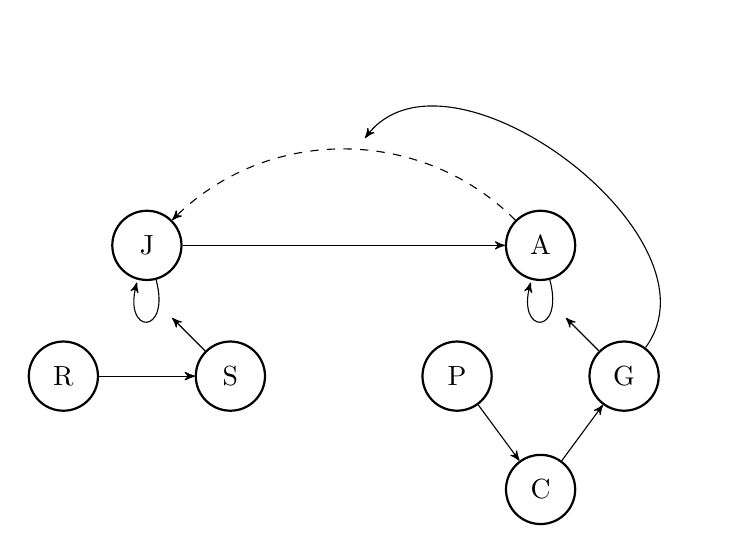
\begin{tikzpicture}[->,>=stealth',auto,thin]
\tikzstyle{every state}=[fill=white,shape=circle,draw,thick,text=black, text centered, text width=0.5cm, align=center]

%\node[state]        (O) [left of=A,node distance=1cm,draw=none,fill=none] {3)};
\node[state]        (A)         {J};
\node[state]		(B) [below of=A,node distance=0.6cm,draw=none,fill=none] {};
\node[state]		(C) [below left of=B,node distance=1.5cm] {R};
\node[state]        (D) [below right of=B,node distance=1.5cm] {S};
\node[state]        (E) [right of=A, node distance=5cm] {A};
\node[state]		(F) [below of=E,node distance=0.6cm,draw=none,fill=none] {};
\node[state]		(G) [below left of=F,node distance=1.5cm] {P};
\node[state]		(I) [below of=F,node distance=2.5cm] {C};
\node[state]        (J) [below right of=F,node distance=1.5cm] {G};
\node[state]        (K) [right of=A,node distance=2.5cm,draw=none,fill=none] {};
\node[state]        (L) [above of=K,node distance=1cm,draw=none,fill=none] {};

\path
(A) edge[loop below] (A)
(C) edge (D)
(D) edge (B)
(C) edge (D)
(A) edge (E)
(E) edge[loop below] (E)
(E) edge[dashed,bend left=-45] (A)
(G) edge (I)
(I) edge (J)
(J) edge[bend right=90, min distance=1.5cm] (L)
(J) edge (F)
;
    \end{tikzpicture}
    \caption{Inter-generational resource transfer model}
\end{subfigure}
\begin{subfigure}{.4\textwidth}
  \centering
  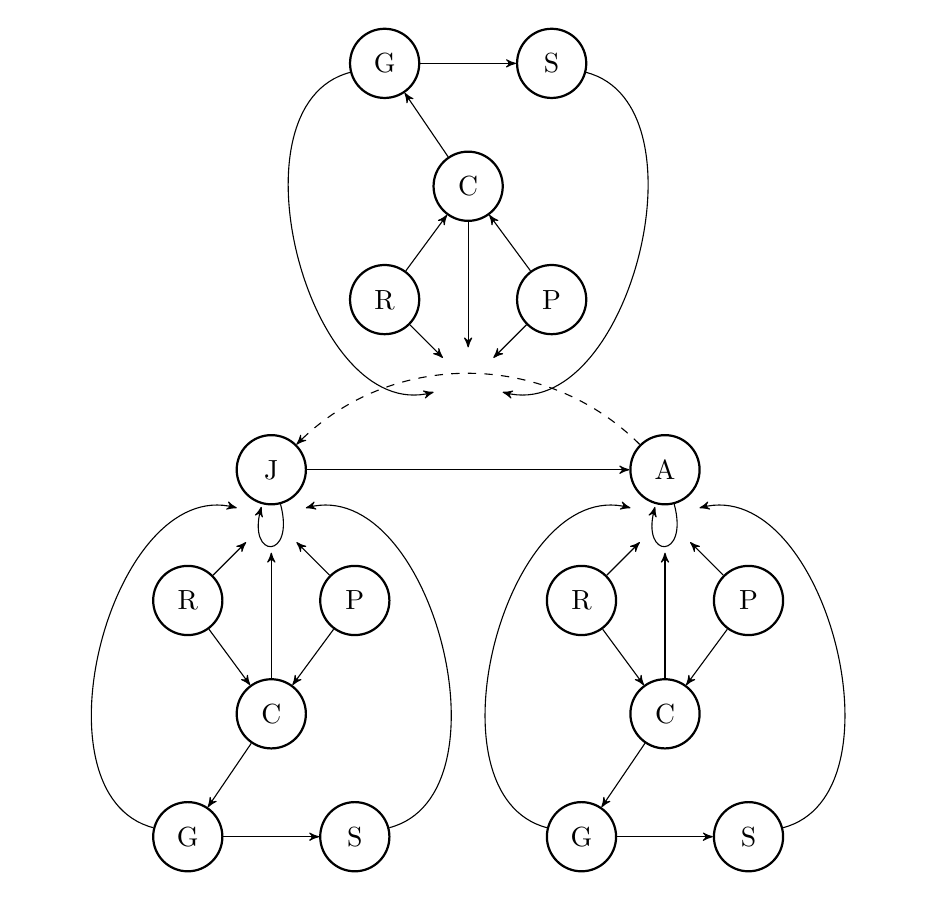
\begin{tikzpicture}[->,>=stealth',auto,thin]
\tikzstyle{every state}=[fill=white,shape=circle,draw,thick,text=black, text centered, text width=0.5cm, align=center]

%\node[state]        (O) [left of=A,node distance=1cm,draw=none,fill=none] {4)};
\node[state]        (A)         {J};
\node[state]		(B) [below of=A,node distance=0.6cm,draw=none,fill=none] {};
\node[state]		(C) [below left of=B,node distance=1.5cm] {R};
\node[state]        (D) [below of=C,node distance=3cm] {G};
\node[state]		(E) [below of=B,node distance=2.5cm] {C};
\node[state]        (F) [below right of=B,node distance=1.5cm] {P};
\node[state]		(G) [below of=F,node distance=3cm] {S};
\node[state]        (H) [right of=A, node distance=5cm] {A};
\node[state]		(I) [below of=H,node distance=0.6cm,draw=none,fill=none] {};
\node[state]		(J) [below left of=I,node distance=1.5cm] {R};
\node[state]		(K) [below of=J,node distance=3cm] {G};
\node[state]		(L) [below of=I,node distance=2.5cm] {C};
\node[state]        (M) [below right of=I,node distance=1.5cm] {P};
\node[state]		(N) [below of=M,node distance=3cm] {S};
\node[state]        (O) [right of=A,node distance=2.5cm,draw=none,fill=none] {};
\node[state]        (P) [above of=O,node distance=1.1cm,draw=none,fill=none] {};
\node[state]		(Q) [above left of=P,node distance=1.5cm] {R};
\node[state]		(R) [above of=Q,node distance=3cm] {G};
\node[state]		(S) [above of=P,node distance=2.5cm] {C};
\node[state]        (T) [above right of=P,node distance=1.5cm] {P};
\node[state]		(U) [above of=T,node distance=3cm] {S};

\path
(A) edge[loop below] (A)
(C) edge (B)
(C) edge (E)
(D) edge[bend right=-90] (B)
(D) edge (G)
(E) edge (B)
(E) edge (D)
(F) edge (B)
(F) edge (E)
(G) edge[bend left=-90] (B)
(A) edge (H)
(H) edge[loop below] (H)
(H) edge[dashed,bend left=-45] (A)
(J) edge (I)
(J) edge (L)
(K) edge[bend right=-90] (I)
(K) edge (N)
(L) edge (I)
(L) edge (K)
(M) edge (I)
(M) edge (L)
(N) edge[bend left=-90] (I)
(Q) edge (P)
(Q) edge (S)
(R) edge[bend left=-90] (P)
(R) edge (U)
(S) edge (P)
(S) edge (R)
(T) edge (P)
(T) edge (S)
(U) edge[bend right=-90] (P)
;

    \end{tikzpicture}
    \caption{Proposed model}
\end{subfigure}

    \caption{Graphical representation of the relationship of resource dynamics with the female human life cycle. Figure 1 represents the embodied capital model \citep{kaplan1996theory}, figure 2 represents the inter-generational resource transfer model \citep{chu2006co}, and figure 3 represents our model. J and A represent juvenile and adult life stages, respectively. The thick arrows between life cycle stages refers to the transition from one stage to the other. Loop arrows below life cycle stages refers to the probability of staying in that stage. The dashed arrows refers to the production of offspring in that life cycle.  The resource dynamics are production (P), consumption (C), receiving (R), giving (G), and storing (S), and the thick arrows represent the relationship among them and the female human life cycle.}
    \label{fig:1}
    
\end{figure}
\end{sidewaysfigure}

\begin{sidewaysfigure}
\begin{figure}[H]
    \centering
    \begin{tikzpicture}[->,>=stealth',auto,thin]
\tikzstyle{every state}=[fill=white,shape=square,draw,thick,text=black, text centered, text width=0.5cm, align=center]

\node[state]		(A) [shape=circle]             {I};
\node[state]		(B) [below of=A,node distance=0.6cm,draw=none,fill=none] {};
\node[state]		(C) [below left of=B,node distance=1.5cm] {R};
\node[state]		(D) [below of=B,node distance=2.5cm] {C};
\node[state]        (E) [below right of=B,node distance=1.5cm,draw=none,fill=none] {};
\node[state]		(F) [below of=E,node distance=3cm] {S};
\node[state]        (G) [right of=A, node distance=5cm,shape=circle] {J};
\node[state]		(H) [below of=G,node distance=0.6cm,draw=none,fill=none] {};
\node[state]		(I) [below left of=H,node distance=1.5cm] {R};
\node[state]        (J) [below of=I,node distance=3cm] {G};
\node[state]		(K) [below of=H,node distance=2.5cm] {C};
\node[state]        (L) [below right of=H,node distance=1.5cm] {P};
\node[state]		(M) [below of=L,node distance=3cm] {S};
\node[state]        (N) [right of=G, node distance=5cm,shape=circle] {A};
\node[state]		(O) [below of=N,node distance=0.6cm,draw=none,fill=none] {};
\node[state]		(P) [below left of=O,node distance=1.5cm] {R};
\node[state]		(Q) [below of=P,node distance=3cm] {G};
\node[state]		(R) [below of=O,node distance=2.5cm] {C};
\node[state]        (S) [below right of=O,node distance=1.5cm] {P};
\node[state]		(T) [below of=S,node distance=3cm] {S};
\node[state]		(U) [right of=N, node distance=5cm,shape=circle]             {RC};
\node[state]		(V) [below of=U,node distance=0.6cm,draw=none,fill=none] {};
\node[state]		(W) [below left of=V,node distance=1.5cm] {R};
\node[state]		(X) [below of=W,node distance=3cm] {G};
\node[state]		(Y) [below of=V,node distance=2.5cm] {C};
\node[state]        (Z) [below right of=V,node distance=1.5cm] {P};
\node[state]		(AA) [below of=Z,node distance=3cm] {S};
\node[state]		(BB) [right of=U, node distance=5cm,shape=circle]             {PR};
\node[state]		(CC) [below of=BB,node distance=0.6cm,draw=none,fill=none] {};
\node[state]		(DD) [below left of=CC,node distance=1.5cm] {R};
\node[state]		(EE) [below of=DD,node distance=3cm] {G};
\node[state]		(FF) [below of=CC,node distance=2.5cm] {C};
\node[state]        (GG) [below right of=CC,node distance=1.5cm] {P};
\node[state]		(HH) [below of=GG,node distance=3cm] {S};
\node[state]		(II) [above of=G, node distance=2.2cm,draw=none,fill=none] {};
\node[state]		(JJ) [above left of=II,node distance=2.2cm] {R};
\node[state]        (KK) [above of=JJ,node distance=3cm] {G};
\node[state]		(LL) [above of=II,node distance=3cm] {C};
\node[state]        (MM) [above right of=II,node distance=2.2cm] {P};
\node[state]        (NN) [above of=MM,node distance=3cm] {S};
\node[state]		(OO) [above right of=N, node distance=3cm,draw=none,fill=none] {};
\node[state]		(PP) [above left of=OO,node distance=2.2cm] {R};
\node[state]        (QQ) [above of=PP,node distance=3cm] {G};
\node[state]		(RR) [above of=OO,node distance=3cm] {C};
\node[state]        (SS) [above right of=OO,node distance=2.2cm] {P};
\node[state]        (TT) [above of=SS,node distance=3cm] {S};

\path
(A) edge[loop below] (A)
(C) edge (B)
(C) edge (D)
(D) edge (B)
(D) edge (F)
(F) edge[bend left=-90] (B)
(A) edge (G)
(G) edge[loop below] (G)
(I) edge (H)
(I) edge (K)
(J) edge[bend right=-90] (H)
(J) edge (M)
(K) edge (H)
(K) edge (J)
(L) edge (H)
(L) edge (K)
(M) edge[bend left=-90] (H)
(G) edge (N)
(N) edge[loop below] (N)
(P) edge (O)
(P) edge (R)
(Q) edge[bend right=-90] (O)
(Q) edge (T)
(R) edge (O)
(R) edge (Q)
(S) edge (O)
(S) edge (R)
(T) edge[bend left=-90] (O)
(N) edge (U)
(U) edge[loop below] (U)
(W) edge (V)
(W) edge (Y)
(X) edge[bend right=-90] (V)
(X) edge (AA)
(Y) edge (V)
(Y) edge (X)
(Z) edge (V)
(Z) edge (Y)
(AA) edge[bend left=-90] (V)
(U) edge (BB)
(BB) edge[loop below] (BB)
(DD) edge (CC)
(DD) edge (FF)
(EE) edge[bend right=-90] (CC)
(EE) edge (HH)
(FF) edge (CC)
(FF) edge (EE)
(GG) edge (CC)
(GG) edge (FF)
(HH) edge[bend left=-90] (CC)
(N) edge[dashed,bend left=-45] (A)
(JJ) edge (II)
(JJ) edge (LL)
(KK) edge[bend left=-90] (II)
(KK) edge (NN)
(LL) edge (II)
(LL) edge (KK)
(MM) edge (II)
(MM) edge (LL)
(NN) edge[bend right=-90] (II)
(U) edge[dashed,bend left=-45] (A)
(PP) edge (OO)
(PP) edge (RR)
(QQ) edge[bend left=-90] (OO)
(QQ) edge (TT)
(RR) edge (OO)
(RR) edge (QQ)
(SS) edge (OO)
(SS) edge (RR)
(TT) edge[bend right=-90] (OO)
\end{tikzpicture}
\caption{Life cycle graph of the human life cycle under different combinations of resource dynamics. I is the newborn stage (i.e. infant), J the sexually immature stage (i.e. juvenile), A the reproductive non-breeding stage (i.e. adult), RC the reproductive career stage, and PR the post-reproductive stage. The thick arrows between life cycle stages refers to the transition from one stage to the other. Loop arrows below life cycle stages refers to the probability of staying in that stage. A newborn is produced either when an individual transition from stage A to RC or when an individual remains in stage RC. The dashed arrows refers to the production of offspring in that life cycle. Resource dynamics (P=production, C=consumption, R=resources received, G=resources given away, S=resources stored) that relate to the timing of life cycle stage transition and offspring production and timing are described with thick arrows among the stage-specific resource production (P), consumption (C), receiving (R), giving (G), and storing (S) and the corresponding life cycle stage.}
    \label{fig:2}
\end{figure}
\end{sidewaysfigure}

\begin{landscape}
    \centering
    \caption{Summary of the different models developed to address the influence of resource availability and sharing dynamics on the female human life cycle}
    \begin{longtable}{ p{0.1\textwidth} p{0.25\textwidth} p{0.25\textwidth} p{0.25\textwidth} p{0.15\textwidth} p{0.1\textwidth} p{0.1\textwidth} p{0.1\textwidth} p{0.1\textwidth} p{0.1\textwidth} p{0.25\textwidth} p{0.25\textwidth} }
    \hline
    Model & Evolutionary pattern & Driver of behavioural change & Modified variables & Outcome variables & Production & Consumption & Receiving & Giving & Storing & Gaps & Reference \\ 
    \hline
    Embodied capital model & Surplus of resource production during adulthood allows the evolution of the female human life cycle & Differences in the allocation of income into the survival and embodied capital of offpsring. & Number of offspring to produce. Resources invested in offspring survival until adulthood. Resources invested in the embodied capital of the offspring. & Fitness (i.e. expected lifetime reproduction = R0) & Income & Individual survival & Income & Reproductive effort (resource transfer from parent to offspring) & Embodied capital & Resource dynamics are coupled as income. Resource transfers towards offspring income and survival (i.e. parental investment) are considered reproductive effort. & \cite{kaplan1996theory,kaplan2000theory,kaplan2003embodied} \\ 
    Pooled energy model & Alloparenting decreases the load of parental investment, allowing overlaping reproductive events. Pooling energy from juveniles, postpones age of sexual maturity, explaining long juvenile periods and slow growth in humans. & Differences in the energy costs and availability for an individual changes the allocation of resources to growth and reproduction, where pooled energy has a buffering effect & Maintenance, production, activity (i.e. labor transfers) & Growth and reproduction & Individual production & Individual consumption & Juveniles receives calories from adult in exchange of low-productivity activity & Adult gives a share of calories to juvenile, to focus on high-productive activities & NA & Transfers are related to a common pool of energy, allowing individuals beyond mother-offspring to be involved & \cite{kramer2010pooled} \\  
    Inter-generational model (I) & Early-life and later-life mortality patterns are because of later age reproductive value and resource transfers & Fertility and resource transfers change the force of selection on mortality, changin the population growth rate (r) & Mortality, fertility, resource dynamics (i.e. production, consumption, transfers) & Stable population growth rate (r) & Individual production & Individual consumption & Negative difference from production$-$consumption & Positive difference from production$-$consumption & NA & Transfers are only directed downwards and modelled as the difference between production and consumption. No storage function. No third generation & \cite{lee2002children,lee2003rethinking,lee2008sociality} \\  
    Inter-generational model (II) & Low mortality co-evolves with downward resource transfers & Changes in resource transfers influence survival and fitness, coevolving more transfers with low mortality. & Maintenance, fertility, growth, resource transfers & Population growth ($\lambda$) & Individual production & Maintenance & Juvenile probability of receiving & Adult probability of giving & Body size & Transfers are only directed downwards. No third generation & \cite{chu2006co} \\  
    Thomas model & Optimal IBIs varies depending on environmental mortality and sibling competition. At high levels of infant mortality, sibling effects become less important, and viceversa. & The probability of having an offspring and its survival depends on the survival probabilities of the adult female as well as the number of siblings, and their weights on child survival (e.g. sibling competition or juvenile help) & Adult female survival and its probability of making it to the next state, the probability of having a child and survives, the wieght of family structure (i.e. number of siblings). & Expected number of offsprings left t years in the future by a female. Interbirth intervals & NA & NA & NA & NA & Transfers are not specified in the model. Sibling effects are based on the competition and helping weighting of earlier offspring (i.e. family structure). No third generation & \cite{thomas2015dynamic} \\  
    Mace model & The decision to have another baby depends on the wealth of the household, the current family size, and the costs of marrying a son or a daughter. Higher fertility is associated with higher wealth and with marrying daughters over sons (sons are more costly). & Changes in the number of camels and the number of children that an adult has influence the decision to have an offspring at time t & Herd size (i.e. wealth) and family size & Expected (at time t) number of children that will be alive at the end of the parents reproductive life (time T) that the parents will have sufficient wealth to marry off. & Wealth & Costs of marriage & NA & NA & Wealth & Transfers are not specified in the model. Resource dynamics are considered only as production and consumption. No third generation &  \cite{mace1996have} \\  
    Price and Jones model & Individuals don't maximize fitness directly, but deal with proximate variables (consumption) where pessimistic (risk-aversion) is the one that alings with fitness maximization & Changes in the decisions of consumption of proximate variables influence variations of age-specific survival and fertility, which influence changes in fitness. & Age-specific survival and fertility. Consumption of proximate variables (i.e. resources) & Fitness (i.e. rate of exponential growth rate of a phenotype a (logarithm of growth rate)) & NA & Consumption of proximate variables & NA & NA & NA & Consumption, resource transfers, and storing are not specified in the model. Only consumption of proximate variables. & \cite{price2020fitness} \\  
    ADP model: somatic state-based & Individuals can develop different phenotypic outcomes depending on changes of a somatic state variable, due to a developmental input, that is linked to a phenotypic outcome. & A phenotype would be adaptive if the developmental input influences the state variable that makes the phenotype advantageous.The alternative phenotype must be adaptive in case the adult environment does not match the developmental input. & Developmental input, the somatic state variable that is associated with the developmental input, and a phenotype. & Fitness & NA & NA & NA & NA & NA & Resource dynamics are not modelled. Only addresses the influence of early conditions (i.e. developmental input) with later phenotypic outcomes. & \cite{nettle2015adaptive} \\  
    ADP model: information & Individuals develop different phenotypic outcomes depending on developmental inputs in earlier stages of the life cycle that forecast adult environment. & A phenotype would be adaptive if the developmental input strongly predicts the adult environment. The alternative phenotype must be adaptive for the alternative adult environment. & Developmental input that predict future environment and the phenotype associated with it. & Fitness & NA & NA & NA & NA & NA & Resource dynamics are not modelled. Only addresses the influence of early conditions (i.e. developmental input) with later phenotypic outcomes. & \cite{nettle2015adaptive} \\
    Our model & Differences in the interacion of resource dynamics (i.e. transfers, production, consumption, and storage) makes individuals to vary their life cycle. Resource transfers have a buffering effect in the variations of the female human life cycle, while production and consumption increase variations. & Changes in the interaction among resource dynamics (e.g. high production and low resource transfer) changes more drastically, or not, the female human life cycle & Resource transfers (i.e. given and recieved), production, consumption, and storage. & Longevity, number of offspring, age at menarche, age at first and last reproduction, age at menopause, interbirth interval. & Stage-specific individual production & Stage-specific individual consumption & Stage-specific probability of receiving & Stage-specific probability of giving & Stage-specific probability of storing &Resource dynamics do not include the influence of previous resource dynamcis into future events, making decisions of the individual be based on the current resources available (produced, consumed, shared, and stored so far). & \\
    \hline
    \end{longtable}
    \label{tab:1}
\end{landscape}

\begin{table}[H]
    \centering
    \caption{References for setting the scenarios in which the individuals will evolve.}
    \begin{tabular}{ l r }
    \hline
    Auxiliary variable & Reference \\ 
    \hline
    Die & \cite{gurven2007longevity} \\  
    Produce & \cite{koster2020life} \\  
    Times receiving & \cite{gurven2004give} \\  
    Receive & \cite{gurven2004give} \\  
    Consume & \cite{kaplan2000theory,pontzer2021daily} \\  
    Store & \cite{bowles2011cultivation} \\  
    Times giving & \cite{gurven2004give} \\  
    Reproduce & \cite{wood2017dynamics} \\  
    Transition & \cite{mulder1989menarche,kramer2010teen,wood2017dynamics,laisk2019demographic} \\
    \hline
    \end{tabular}
    \label{tab:2}
\end{table}

\clearpage

\bibliographystyle{apalike}
\bibliography{optimal_ref}

\end{document}
